\begin{figure}[htbp]
    \centering
    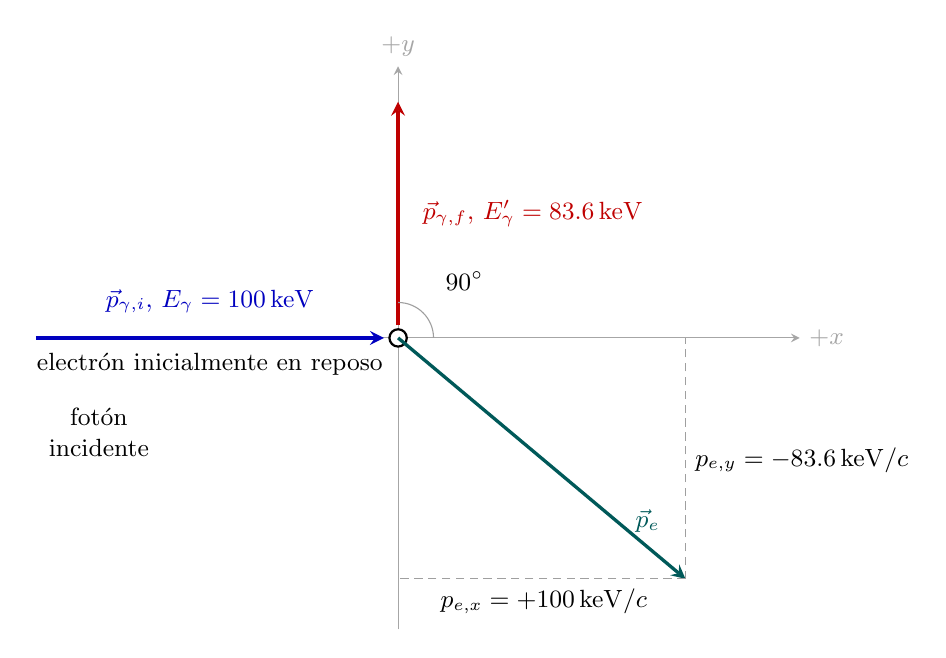
\begin{tikzpicture}[>=stealth, every node/.style={font=\small}]
        \draw[->,gray!70] (-0.45,0) -- (5.1,0) node[right] {$+x$};
        \draw[->,gray!70] (0,-3.7) -- (0,3.45) node[above] {$+y$};
        \filldraw[fill=white,draw=black,thick] (0,0) circle (0.11);
        \node[below left=2pt] at (0,0) {electrón inicialmente en reposo};

        \draw[->,very thick,blue!75!black] (-4.6,0) -- (-0.18,0)
            node[midway,above=5pt] {$\vec p_{\gamma,i}$, $E_\gamma=100\,\mathrm{keV}$};
        \draw[->,very thick,red!75!black] (0,0.16) -- (0,3.0)
            node[midway,right=5pt] {$\vec p_{\gamma,f}$, $E'_\gamma=83.6\,\mathrm{keV}$};
        \draw[->,very thick,teal!70!black] (0,0) -- (3.65,-3.06)
            node[pos=0.76,right=3pt] {$\vec p_e$};
        \draw[densely dashed,gray!75] (3.65,-3.06) -- (3.65,0);
        \draw[densely dashed,gray!75] (3.65,-3.06) -- (0,-3.06);
        \node[below] at (1.85,-3.06) {$p_{e,x}=+100\,\mathrm{keV}/c$};
        \node[right] at (3.65,-1.55) {$p_{e,y}=-83.6\,\mathrm{keV}/c$};
        \draw[gray!75] (0.45,0) arc[start angle=0,end angle=90,radius=0.45];
        \node[above right] at (0.48,0.48) {$90^\circ$};
        \node[align=center] at (-3.8,-1.2) {fotón\\incidente};
    \end{tikzpicture}
    \caption{Geometría de la dispersión Compton a $90^\circ$. La conservación vectorial del momento, $\vec p_e=\vec p_{\gamma,i}-\vec p_{\gamma,f}$, fija el retroceso del electrón y sus componentes.}
    \label{fig:compton-recoil}
\end{figure}